\documentclass[a4paper, 11pt]{article}

\usepackage[english]{babel}
\usepackage[utf8]{inputenc}
\usepackage[T1]{fontenc}
\usepackage{graphicx}
\usepackage{color}
\usepackage{amsmath,amssymb}
\usepackage{rotating}
\usepackage{layaureo}
\usepackage{booktabs}
\usepackage{varioref}
%\usepackage{subfigure}
\usepackage{listings}
\usepackage{wrapfig}
\usepackage{siunitx}
\usepackage{physics}
\usepackage{subcaption} 
\usepackage{subfloat}
\usepackage{caption}
\usepackage{gensymb}
\usepackage{mhchem}
\usepackage{afterpage}

\sisetup{output-decimal-marker={.}}

\author{Jakub Skowronski \& Alessandro Compagnucci}
\title{GALTRACE: }

\begin{document}

\maketitle

\clearpage

\tableofcontents

\clearpage

\section{Introduction}

One of the modern detection methods, offering identification of the reaction
products with very low energy, is the Pulse Shape Analysis (PSA). This method
can be applied to the signals from silicon detectors. As shown by Mengoni et
al.~\cite{mengoni}, in the case of the TRacking Array for Charged Ejectile (TRACE) array, consisting
of 200-$\mu$m thick silicon modules and divided in 60 separately read pixels,
the identification of the \ce{^{1,2,3} H} isotopes can be easily obtained.
In addition, the separation between \ce{^3 He} and \ce{^4 He} was also
observed. This proved that the thin detector, with the uniformity guaranteed
by the fine pad segmentation, may provide a good particle discrimination when
the PSA technique is applied.

\bigbreak

The experimental application choosen to test the detector is the reconstruction of the excitation energy of \ce{^19 O},
a neutron-rich nuclei, by the detection of the evaporated protons,
isotropically emitted in the center of mass reference system with an estimated total cross section of about $50$ mb. For this purpose, a segmented light
charged particle array was employed, made of 4$\Delta$E-E telescopes from the
TRACE project, positioned at backward angles with respect to
the beam direction, coupled to the GALILEO detection system~\cite{galileo}.
If successful, this would allow to investigate the structure of light reaction
products, such as \ce{Be}, \ce{B}, \ce{C}, \ce{N} and \ce{O} by a direct
measurement of their energy, position, mass, and charge.

\bigbreak

This report presents the initial stages of the TRACE detector calibration
with 3 peaks from 3 different $\alpha$ source (\ce{^239 Pu}, \ce{^241 Am},
\ce{^244 Cm}), the construction of the electronical chain for the data
acquisition and the development of a Neural Network (NN) model, based on the
Pulse Shape Anlaysis (PSA) of the signal from the detector, in order to
identify the proton and $\alpha$ particles emmited by the daughter nuclei
produced during the experiment. Finally, an initial and brief attempt for the
$\gamma-\gamma$ coincidences identification is presented.

\clearpage

\section{Physical Motivation}

The knowledge of the nuclide chart far from the stabilty valley is one of the
fundamental topics for the nuclear structure studies, as it could hopefully
lead to the comprehension of the nuclear force, which is responsible both for
the abundance of stable nuclei and for weakly bound systems.
Nuclei can be formed in multiple diffrent combinations of protons and neutrons.
However, because of the fundamental forces and symmetries of Nature, not all
combinantions are stable and bound.

\bigbreak

The nuclear landscape show more than $3000$ of nuclei that are expected to be
bound by the strong force. Among these, less than $300$ are stable, while the
others are bound against the emission of protons and neutrons, or against the
$\beta$-decay, in which a proton decays into a neutron (or vice versa). Some
of the unstable nuclei are long-lived and found on Earth, some are produced
experimentally while other thousands, far from stabiity, are still undetected.
Consequently, from the multitude of nuclei that may exist and that could have
been formed i.e.\ in violent stellar explosions, only a very limited number
have been studied.

\bigbreak

\begin{figure}[h]
  \centering
  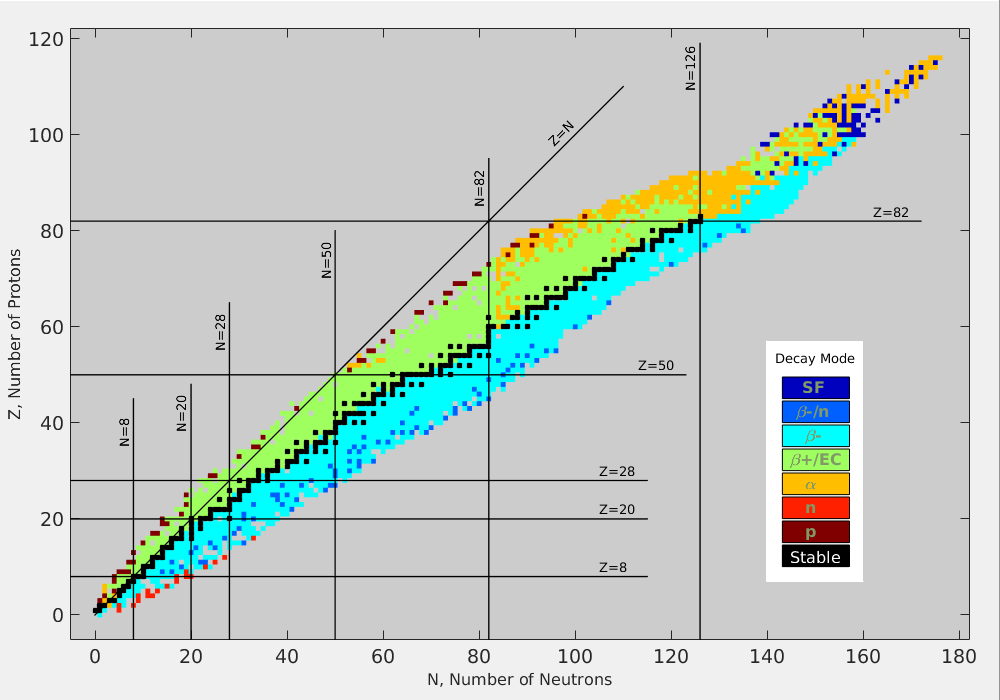
\includegraphics[scale=.35]{img/DecayModeNuDat2.png}
  \caption{The nuclide landscape}
  \label{nucl}
\end{figure}

\bigbreak

In particular, the neutron-rich light isotopes of \ce{Be}, \ce{C}, \ce{O} and
\ce{Ne} offer an extremely fertile ground for nuclear structure studies far
from stabilty region. On one hand, they may serve as examples of nuclear
clustering: for instance, in \ce{^12 C} many states have a well-established
$\alpha$-cluster structure. On the other hand, they exhibit features of
shell-model nuclei in which the impact of the continuum on the shell structure
has to be considered. This characteristics is clearly visible in \ce{^19 O},
in which a comprehensive analysis of the known excitations provides evidence
for states with single-particle structure and states which have strong
$\alpha$-clustering and form rotational bands.

\bigbreak

Description of excitations of the first type involve the standard nuclear
Shell Model (SM), which is an a priori approach; here, the degrees of freedom
are the valence protons and neutrons moving in specific shells – this model
cannot predict cluster states.
The second group of states can be treated with cluster models, which, in turn,
are a posteriori approaches that assume effective building blocks (clusters).
Both these approaches present, however, rather disjointed and not fully
consistent physical descriptions as they assume the nucleus to be a closed
quantum system that is completely isolated from the subspace of scattering and
decay channels. It is clear that a comprehensive understanding of low-energy
excitations in neutron-rich oxygen isotopes cannot emerge from such a picture.

\bigbreak

A significant step forward in creating the link between the SM approach and
the cluster approach to the structure of light nuclei was recently
made~\cite{oko:cluster}~\cite{oko:origin}.
It was showed that the mixing of SM eigenstates, induced by the external
coupling to the decay channel(s), profoundly impacts the nature of SM
eigenstates lying near particle-decay thresholds. 
It was concluded that the mixing of SM eigenstates (with the same quantum
numbers) via the continuum explains:

\begin{itemize}
\item the emergence of clustering leading to the appearance of
collective/cluster states located near the corresponding particle decay
thresholds
\item a gradual disappearance of charged-particle clustering in heavier nuclei
\end{itemize}

The $\alpha$-cluster states, being the best manifestation of the near-threshold
clustering phenomenon, cannot, however, be calculated with the SMEC Model
approach yet. The other class of near-particle-decay threshold states are
states lying close to the nucleon-decay thresholds - they are also
commonly observed in light nuclei. Here, the degree of collectivization can be
predicted by the SMEC Model, but the clear comparison with experiment has not
yet been done. 

\bigbreak

In this context, the measurement of electromagnetic decay from unbound
near-threshold states in neutron-rich systems, which could prove the predicted
near-threshold collectivization phenomenon by the observation of the increase
of electromagnetic transitions probability, would represent a breakthrough.
At present, such information is almost totally missing, as a consequence of
very low  $\gamma$-decay branchings, of the order of $10^{-3}$-$10^{-4}$ and
even lower. The studies call then for the use of very selective reaction
mechanisms and $\gamma$ spectrometers, in order to enhance the sensitivity to
the population of unbound states and their electromagnetic decays.



\subsection{Silicon detectors}

Silicon is the dominant semiconductor material used in the production of
detectors for particle physics. The moderate band gap between the conduction
and the valence band of $1.12$ eV is large compared to the thermal
energy at room temperature of $25.9$ meV. Therefore cooling is necessary
only in ultra-low noise applications or when required to mitigate radiation
damage. The detection of minimum ionizing particles (MIP) is based on
ionisation or excitation of atoms in the medium caused by the passage of
charged particles. The energy required to create an electron-hole (e-h) pair
is $3.6$ eV yielding an ionization of about 80 (e-h)/$\mu$m. Thus silicon
detector can be quite thin compared with gaseous detectors. The typical
thickness used in high-energy physics varies between 100 and 500 $\mu$m.

\bigbreak

\begin{figure}[h]
  \centering
  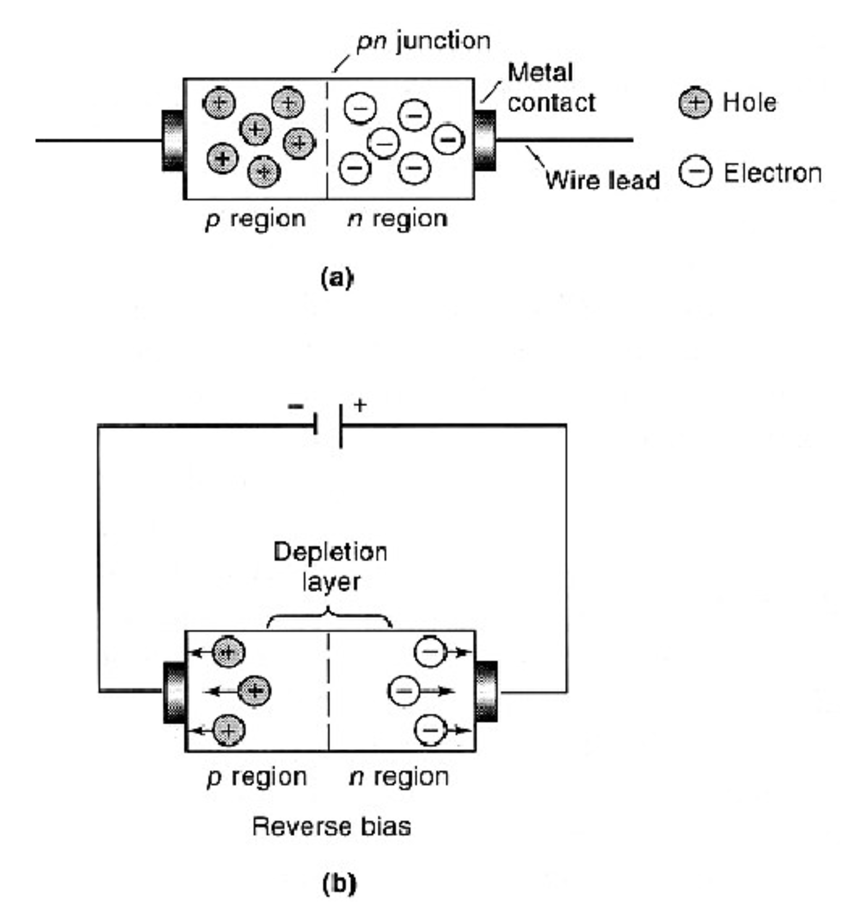
\includegraphics[scale=.25]{img/depletion.png}
  \caption{$p$-$n$ junction}
  \label{chain}
\end{figure}

\bigbreak

In intrinsic silicon there are $\sim 10^9$ free charge carriers at room
temperature but only $\sim 2 \times 10^4$ electrons are induced by a MIP
traversing 300 $\mu$m. Therefore a MIP signal would be lost among the large
number of free charge carriers. The operation of silicon detectors requires
sensors to be fully or partially depleted of free charge carriers. This can
be achieved by using $p$-$n$ junctions operated in reverse bias. Silicon sensors
are often fabricated on $n$-type bulk by adding a type V material, like
phosphorus \ce{P} (donor impurity) to silicon. Donor impurities provide an
excess of electrons charge carriers. Similarly a $p$-type material can be
realized by adding type III material like boron \ce{B} (acceptor impurities)
that yields an excess of holes as majority charge carriers. Typical doping
concentration used in $n$-bulk silicon sensors are of the order of
$1012$ cm$^{-3}$. The full depletion voltage V$_{\textup{FD}}$=D/2$\varepsilon
\mu \zeta$ depend on the thickness D, the resistivity $\varepsilon$, the
carrier mobility $\mu$, and the shape of the junction $\zeta$.

\bigbreak

\subsection{TRACE detector}

The TRacking Array for light Charged particle Ejectiles (TRACE) is a silicon
detector designed for fusion-evaporation and direct nuclear reactions.
The material, the thickness, the segmentation and a basic geometry have been
simply estimated by empirical considerations, while the final prototype was
chosen among the various geometries by the simulation of their performances
and comparison with already existing detector ancillaries (EUCLIDES, MUST2,
TIARA).

\bigbreak

\begin{figure}[h]
  \centering
  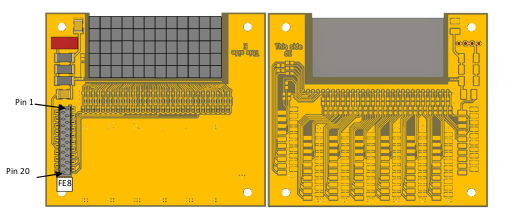
\includegraphics[scale=.65]{img/trace_e.png}
  \caption{TRACE detector (E configuration)}
  \label{chain}
\end{figure}

\begin{figure}[h]
  \centering
  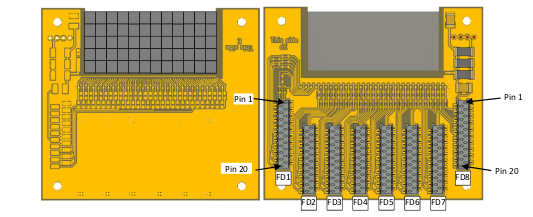
\includegraphics[scale=.65]{img/trace_de.png}
  \caption{TRACE detector (dE configuration)}
  \label{chain}
\end{figure}

\bigbreak

Silicon, for its transparency, energy resolution, moderate cost and
well known properties is chosen as a good compromise for the required
applications. Based on the efficiency criterion, particles dynamics ($\sim$
$100$ MeV for alpha particles and $25$ MeV for protons) and technological
constraints, the thickness of the detector has been chosen to be $150$ $\mu$m
and $1.5$ mm for the $\Delta$E and E layers respectively. The $4 \times 4$ mm
60 pad segmentation has been established from the requirement to have a uniform
counting rate ($20$ kHz maximum) when using high intensity beams and a good
angular resolution ($\sim 2^\circ$), necessary to perform momentum
discrimination in transfer reactions and a good Doppler correction. The pad
has been preferred to the strip segmentation due the expected smaller
electronics noise. The detector, realized on a Rogers 4003c substrate,
incorporates the load resistances and the power supply filtering. A clever
implementation allows for different usages with a signle physical board.
Populating the board on one side connects the detector as $\Delta$E, while
populating on the other side connects the detector as E.


\clearpage

\section{Experimental Setup}

 \subsection{Electronic chain linearity}

In order to prepare the data acquistion system, the entire electronical chain
was tested beforehand. In fact it is crucial that the response of each
electronic device used behaves linearly, as the information about the energy
of the incident particle must be univocally extracted at the end of the chain.

\bigbreak

\begin{figure}[h]
  \centering
  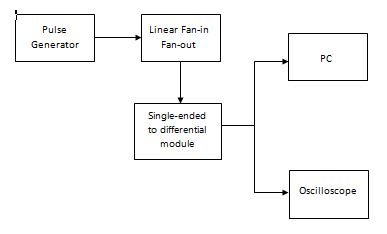
\includegraphics[scale=.6]{img/electronic_chain_diagram.JPG}
  \caption{The electronic chain}
  \label{chain}
\end{figure}

\bigbreak

The setup used is shown in Fig.~\ref{chain}. The output of a pulse generator (\num{100} ns square pulse of variable amplitude) is fed into a Fan-In Fan-Out module which reproduces the same signal for 12 channels. The signals are transmitted
to the single-ended-to-differential (SeDiff) modules, which permit long
connections to the digitizers rack. The SeDiff modules are built around the
AD8139 integrated operational amplifier and convert the single-ended signals
in differential ones. These boards have been designed at the INFN LNL and are
compliant with the preamplifier standards in terms of dynamic range, bandwidth
and noise.

\bigbreak



\bigbreak

\begin{figure}[h]
  \centering
  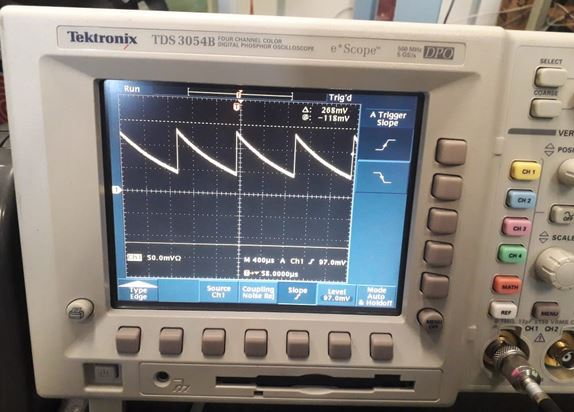
\includegraphics[scale=.35]{img/test_signal_oscilloscope.JPG}
  \caption{The output signal from the differential amplifier board, as seen on the oscilloscope.}
  \label{osc}
\end{figure}

\bigbreak

The signal from the pre-amiplifier is given to a 100 MHz 14-bit resolution digitizer throught a MDR-26 connector.
The trapezoidal filter was applied to the signal through an FPGA with its charateristics \emph{rise time} and \emph{flat top width} parameters (Moving Windows Analysis)~\cite{salathe}. This step is crucial because the height of the peak from the pre-amplifier board will be directly proportional to the energy of the incident particle in the detector. In the exponential curve of the signal, the amount of the time peak is present is very small and the peak detection is made difficult. By the differentiation of the signal, it is possibile to obtain the peak precisely and thus a trapezoidal signal is obtained. 
Hence, the height of the trapezoidal filter with the right parameters gives the information on the maximum of the peak available for longer time.

\bigbreak

The output of the trapezoidal filter is then sampled throught the acquisition software that also control the MWA variables. The software records the amplitude of the output and saves it into different channels during the time of the acquisition. A software, called TKT, is used to perform the fit on the peak obtained for the different pulse amplitude. 

\bigbreak

The linearity of the response of the boards is checked fitting the data obtained versus the voltage given as input to the preamplifier and checking the residuals plot as in Fig.~\ref{calib:plot:1} for all the 24 channels on the board.

\bigbreak

\begin{figure}[th]
  \centering
  \begin{minipage}[b]{0.45\textwidth}
    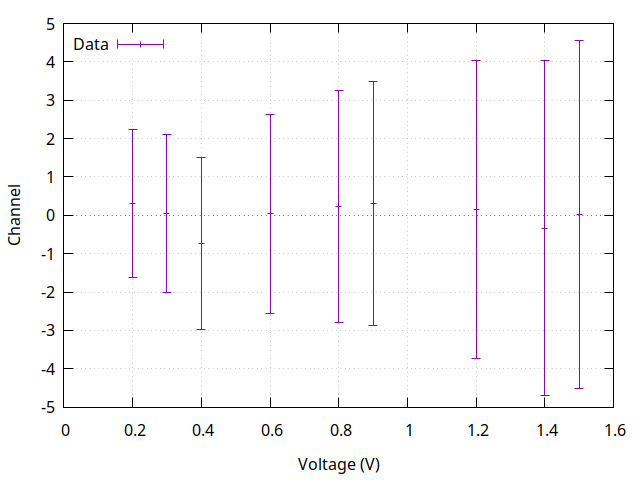
\includegraphics[width=\textwidth]{img/fourth_board_line/data_1/calib_0.png}
    \caption{Residual Plot for the the fit on the first channel on the tested board}
    \label{calib:plot:1}
  \end{minipage}
  \hfill
  \begin{minipage}[b]{0.45\textwidth}
  \begin{tabular}{lll}
    Voltage (V) & Channel & $\sigma$ \\
    \midrule
    0.2 & \num{343.1} & 1.9 \\
    0.3 & \num{519.5} & 2.1 \\
    0.4 & \num{695.4} & 2.2 \\
    0.6 & \num{1049.5} & 2.6 \\
    0.8 & \num{1403.0} & 3.0 \\
    0.9 & \num{1579.8} & 3.2 \\
    1.2 & \num{2109.6} & 3.9 \\
    1.4 & \num{2462.4} & 4.4 \\
    1.5 & \num{2639.5} & 4.5 \\
    \bottomrule
  \end{tabular}
  \caption{Data for the fit}
  \label{calib:1}
  \end{minipage}
\end{figure}

\bigbreak

All the channels gave fairly similar results, therefore confirming the linearity of the response of the electronic chain and a good behavior of the differential board tested.

\subsubsection{Cabling Problem}

After the data acquisition period, a problem with digitizer cabling was
discovered. In fact the two digitizer used for the TRACE detector
(\textit{gal09} and \textit{gal10}) did not use the same MDR cables. All the
channels, apart from 17 to 24 ones of the \textit{gal10}, were connected through
high-end AGATA 10m MDR/MDR cables used by previous experiment. As there were
not enough cables, all the others channels were connected through home made
MDR cables constructed in the LNL laboratory specifically for this experiment.

\bigbreak

In the Fig.~\ref{cable} it is possible to see the differences in the Pulse
Shape of the signals from different types of cables, which are enumerated in
the Tab.~\ref{cables}. As the analysis is made using the Pulse Shape Analysis
(PSA), small differences in the signal propagation has to be taken into
account when calculating the discriminating variables. In fact, as it is clear
from the plot, the rise time and the maximum derivative of the signal will be
different for different types of cable, thus preventing the use of the same
cuts and the same Neural Network model for the PSA.

\bigbreak

\begin{figure}[h]
  \centering
  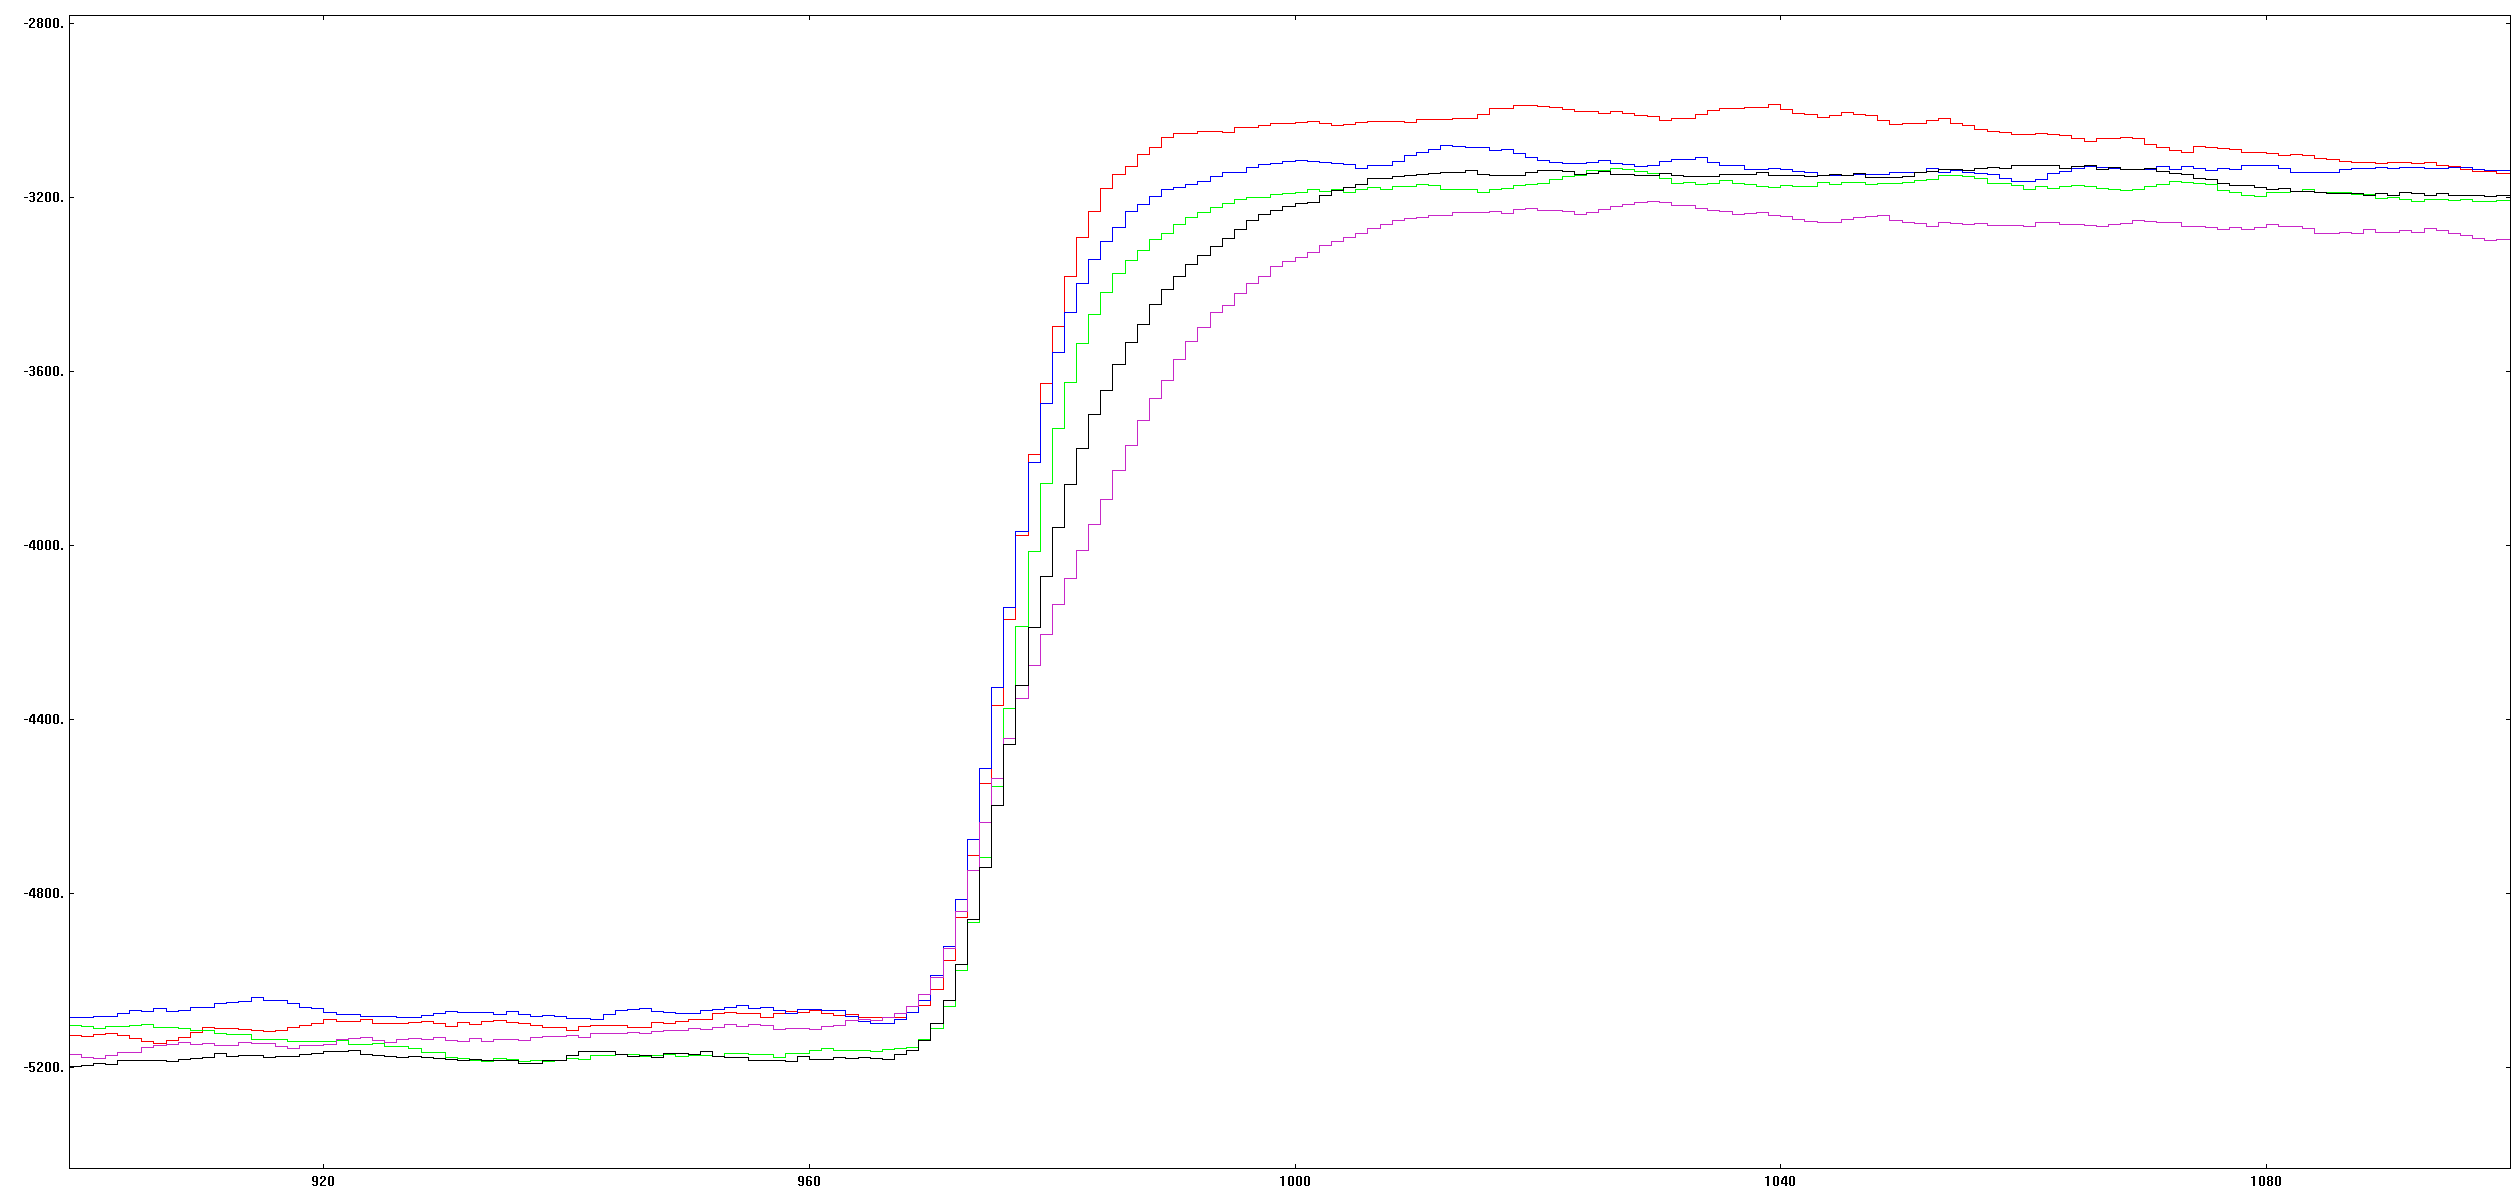
\includegraphics[scale=.16]{img/cabling.png}
  \caption{TRACE signals from different cable type.}
  \label{cable}
\end{figure}

\begin{figure}[h]
  \begin{tabular}{ll}
    Signal Color & Cable \\
    \midrule
    Red & GALILEO 0.8m MDR/MDR \\
    Blue & AGATA 10m MDR/MDR \\
    Green & AGATA 10m MDR/MDR (previous generation 3M cable) \\
    Magenta & Home made MDR flat cables \\
    Black & New cable for TRACE \\
    \bottomrule
  \end{tabular}
  \caption{Legend for Fig.~\ref{cable}.}
  \label{cables}
\end{figure}

\bigbreak

In order to make up for this, the \textit{gal10} 17-24 channels were analyzed
separately, making different cuts and creating a specific Neural Network model
for those. In this way it is possible to discriminate successfully the
protons and $\alpha$ signals also for channels connected through different MDR
cables.

\clearpage

\subsection{Testing the TRACE detector}

In order to test the TRACE detector along with its preamplifier, it was put in a vacuum chamber, with a $\alpha$ source (Fig.~\ref{trace_chamber}).

\begin{figure}[h]
  \centering
  \includegraphics[scale=.05]{img/trace_chamber.jpg}
  \caption{The TRACE detector inside the chamber along with its preamplifier boards and the alpha source.}
  \label{trace_chamber}
\end{figure}

\bigbreak

To connect the integrated charge-sensitive pre-amplifiers to the TRACE silicon detector prototypes a custom board was designed and realized. Each board can host 2 ASIC pre-amplificators with 8 channels each. The ASICS can be reconfigured using different soldering in order to accept the back channel. As each detectors is segmented in 60 pads of 4 mm$^2$, a total of 4 pre-amplification boards are required by one telescope.
The amplified signals is going out of the chamber via a flat cable connected to a FISCHER 27-pins connectors feedthrough making the bridge between the reaction chamber under vacuum ($10^{-3}$ mbar) and the laboratory. Outside of the chamber, from each FISCHER connector, the cables are divided in two 12-pins MOLEX connectors mounted on the Single-ended-to-differential modules. From here the signal goes directly to the 14-bits 100 MHz digitizer for the GALILEO array using MDR-26 connectors and 10 m cables.

\bigbreak

The acquisition is triggered by the back portion of the detector, which is connected as Channel 0 of the digitizer, and it is performed as described in the former section. The resolution is tested using the three peaks of different sources (Tab.~\ref{peaks}). In Tab.~\ref{res:peaks:cab1} and Tab.~\ref{res:peaks:cab2} it is possible to see fit results for the $\alpha$ peaks for 2 different cables.

\begin{figure}[th]
  \centering
 \begin{tabular}{lc}
    Source & $E_\alpha$ (MeV)  \\ 
    \midrule
    \ce{^239Pu} & 5.1566  \\
    \ce{^241Am} & 5.4856  \\
    \ce{^244Cm} & 5.8048 \\
    \bottomrule
  \end{tabular}
  \caption{The predominant peaks from the triple-alpha source.}
  \label{peaks}
\end{figure}

\begin{figure}[h]
  \centering
  \begin{minipage}[b]{0.45\textwidth}
    \centering
  \begin{tabular}{ll}
    Energy (keV) & FWHM (keV) \\
    \midrule
    5150 & \num{29} \\
    5485 & \num{27} \\
    5804 & \num{25} \\
    \bottomrule
  \end{tabular}
  \caption{3-$\alpha$ peaks (cable 1)}
  \label{res:peaks:cab1}
  \end{minipage}
  \hfill
  \begin{minipage}[b]{0.45\textwidth}
    \centering
  \begin{tabular}{ll}
    Energy (keV) & FWHM (keV) \\
    \midrule
    5153 & \num{32} \\
    5485 & \num{27} \\
    5805 & \num{22} \\
    \bottomrule
  \end{tabular}
  \caption{3-$\alpha$ peaks (cable 2)}
  \label{res:peaks:cab2}
  \end{minipage}
\end{figure}

In Fig.~\ref{res:am}, Fig.~\ref{res:pu} and Fig.~\ref{res:cm} results of the calibration for different channels of the detector are shown. They are overral good throughout all the tested channels.

\begin{figure}[h]
  \centering
  \begin{minipage}[b]{0.45\textwidth}
  \vspace{5mm}
    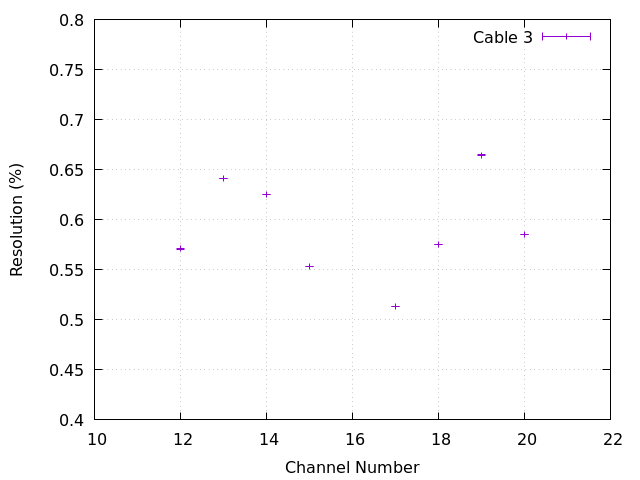
\includegraphics[width=\textwidth]{img/plot/am/3_res_am.png}
    %\caption{Resolution vs Channel}
    \label{res:am3}
  \end{minipage}
  \hfill
  \begin{minipage}[b]{0.45\textwidth}
    \begin{tabular}{lll}
      DAQ Channel & Resolution (\%) & $\sigma$ \\
      \midrule
      12 & \num{0.5708} & 0.0002 \\
      13 & \num{0.6413} & 0.0003 \\
      14 & \num{0.6253} & 0.0003 \\
      15 & \num{0.5535} & 0.0002 \\
      17 & \num{0.5131} & 0.0002 \\
      18 & \num{0.5752} & 0.0002 \\
      19 & \num{0.6646} & 0.0003 \\
      20 & \num{0.5854} & 0.0002 \\
      \bottomrule
    \end{tabular}
    \label{res:plot:am3}
  \end{minipage}
  \caption{Energy resolution (\%) of the TRACE detector for \ce{^241Am} peak.}
  \label{res:am}
\end{figure}

\begin{figure}[h]
  \centering
  \begin{minipage}[b]{0.45\textwidth}
  \vspace{5mm}
    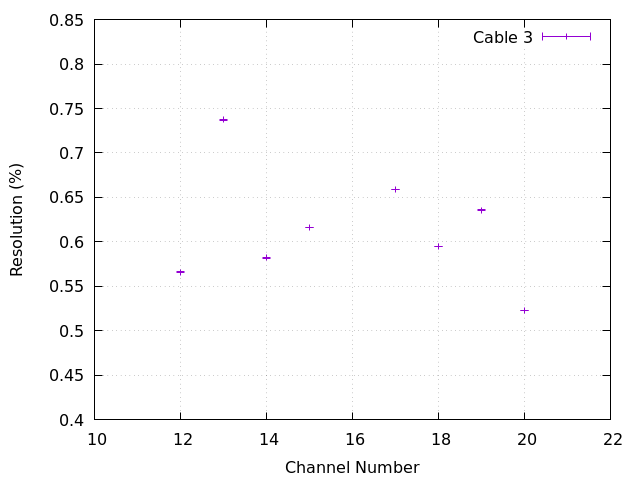
\includegraphics[width=\textwidth]{img/plot/pu/3_res_pu.png}
    %\caption{Resolution vs Channel}
    \label{res:pu3}
  \end{minipage}
  \hfill
  \begin{minipage}[b]{0.45\textwidth}
  \begin{tabular}{lll}
    DAQ Channel & Resolution (\%) & $\sigma$ \\
    \midrule
    12 & \num{0.5661} & 0.0003 \\
    13 & \num{0.7371} & 0.0003 \\
    14 & \num{0.5821} & 0.0003 \\
    15 & \num{0.6160} & 0.0003 \\
    17 & \num{0.6587} & 0.0003 \\
    18 & \num{0.5947} & 0.0003 \\
    19 & \num{0.6359} & 0.0003 \\
    20 & \num{0.5228} & 0.0002 \\
    \bottomrule
  \end{tabular}
  \label{res:plot:pu3}
  \end{minipage}
  \caption{Energy resolution (\%) of the TRACE detector for \ce{^239Pu} peak.}
  \label{res:pu}
\end{figure}

\begin{figure}[h]
  \centering
  \begin{minipage}[b]{0.45\textwidth}
  \vspace{5mm}
    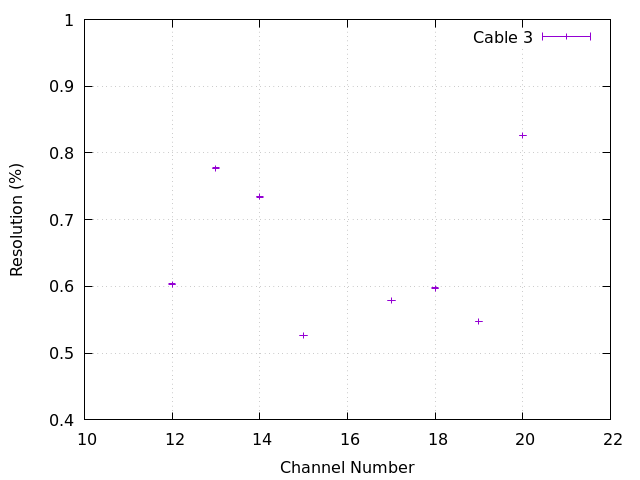
\includegraphics[width=\textwidth]{img/plot/cm/3_res_cm.png}
    %\caption{Resolution vs Channel}
    \label{res:cm3}
  \end{minipage}
  \hfill
  \begin{minipage}[b]{0.45\textwidth}
  \begin{tabular}{lll}
    DAQ Channel & Resolution (\%) & $\sigma$ \\
    \midrule
    12 & \num{0.6036} & 0.0003 \\
    13 & \num{0.7772} & 0.0004 \\
    14 & \num{0.7342} & 0.0004 \\
    15 & \num{0.5262} & 0.0002 \\
    17 & \num{0.5789} & 0.0003 \\
    18 & \num{0.5976} & 0.0002 \\
    19 & \num{0.5472} & 0.0002 \\
    20 & \num{0.8266} & 0.0002 \\
    \bottomrule
  \end{tabular}
  \label{res:plot:cm3}
  \end{minipage}
  \caption{Energy resolution (\%) of the TRACE detector for \ce{^244Cm} peak.}
  \label{res:cm}
\end{figure}

\clearpage

\subsection{GALTRACE experiment}

The experiment was performed in July 2019 at the Legnaro National Laboratory
(Italy) \cite{kuba:compa}. A \ce{^13C} beam, with an energy of $23$ MeV and an
intensity around $1$ pnA was directed on a $0.1$ mg/cm thick \ce{^19 F} -
\ce{^7 Li} target (on a \ce{^12 C} substrate). Two TRACE silicon detectors
were placed inside the GALILEO HPGe array scattering chamber. Inside the
chamber, the detectors were connected with a short cable to a
16-channel charge-sensitive preamplifier, designed at INFN Milano~\cite{strano}.

\bigbreak

The chain of the digital acquisition allowed to collect the signals (“traces”)
digitized by the 100 MHz sampling module. The length of the recorded trace was
1 $\mu$s, giving 100 points, at every 10 ns each. This length of the traces
was chosen to assure recording the full rise time on the one hand and at the
same time minimize the amount of written data. The signals were recorded,
digitized and afterwards processed to extract the relevant observables. The
placement of the TRACE module in the chamber with the ohmic side facing the
reaction products was important to enhance the PSA capability.

\bigbreak

The trigger of the TRACE acquisition, obtained in this case from a digital
leading edge discriminator embedded in the module, was the signal from the
common electrode (“BACK”). The signals from the pads were collected only if
the BACK signal was present.



\clearpage

\section{GALTRACE detector}

\subsection{TRACE Linearity}
 
\subsection{TRACE Calibration \& Resolution}

\begin{figure}[h]
  \centering
  \begin{minipage}[b]{0.45\textwidth}
    \centering
  \begin{tabular}{ll}
    Channel & FWHM \\
    \midrule
    5150 & \num{29} \\
    5485 & \num{27} \\
    5804 & \num{25} \\
    \bottomrule
  \end{tabular}
  \caption{3-$\alpha$ peaks (cable 1)}
  \label{res:peaks:cab1}
  \end{minipage}
  \hfill
  \begin{minipage}[b]{0.45\textwidth}
    \centering
  \begin{tabular}{ll}
    Channel & FWHM \\
    \midrule
    5153 & \num{32} \\
    5485 & \num{27} \\
    5805 & \num{22} \\
    \bottomrule
  \end{tabular}
  \caption{3-$\alpha$ peaks (cable 2)}
  \label{res:peaks:cab2}
  \end{minipage}
\end{figure}

\clearpage

\section{Data Analysis}

\subsection{ROOT Analysis}

The binary data from the DAQ acquisition was analyzed through a C++ code
implemented in a ROOT framework~\cite{root}.

The Pulse Shape Analysis (PSA) were performed directly on the binary data, as,
by doing thus, it is not necessary to save the signal pulse as a ROOT variable
and a further analysis can be facilitated. The \num{100} ns long stamps of the
signal, saved by the digitizer, were used to obtain two discriminating
variables, that describe fully the important features of the pulse signal for
the proton and $\alpha$ identification: $\tau _{\textup{rise}}$ and
$i_{\textup{max}}$, which represent, respectively, the rise time and maximum
derivative of the signal.

In order to calulcate the two, the following algorithms were used:

\begin{itemize}

\item For the rise time, $\tau _{\textup{rise}}$, the difference between the moment when the pulse is at
  70\%, $t_{0.7}$, and when it is at 30\%, $t_{0.3}$ is considered.
  In order to calculate it, the maximum value of the signal, $V_{\textup{max}}$,
  was obtained as the mean of 3 highest values found. Then, two nearest points
  to 30\% (and 70\%) of the signal were found, in order to perform a two-point
  linear interpolation. Then the $t_{0.3}$ (and $t_{0.7}$) is found from the
  interpolating function as the time when the signal height is at
  $0.3 V_{\textup{max}}$
  (and $0.7 V_{\textup{max}}$).
\item For the maximum derivative of the pulse, $i_{\textup{max}}$, 
  the interpolation of the Pulse Shape was performed using a ROOT class,
  called TSpline3, and 5 highest values of its derivative are used for the
  mean value which is the $i_{\textup{max}}$.

\end{itemize}

\begin{figure}[h]
  \centering
  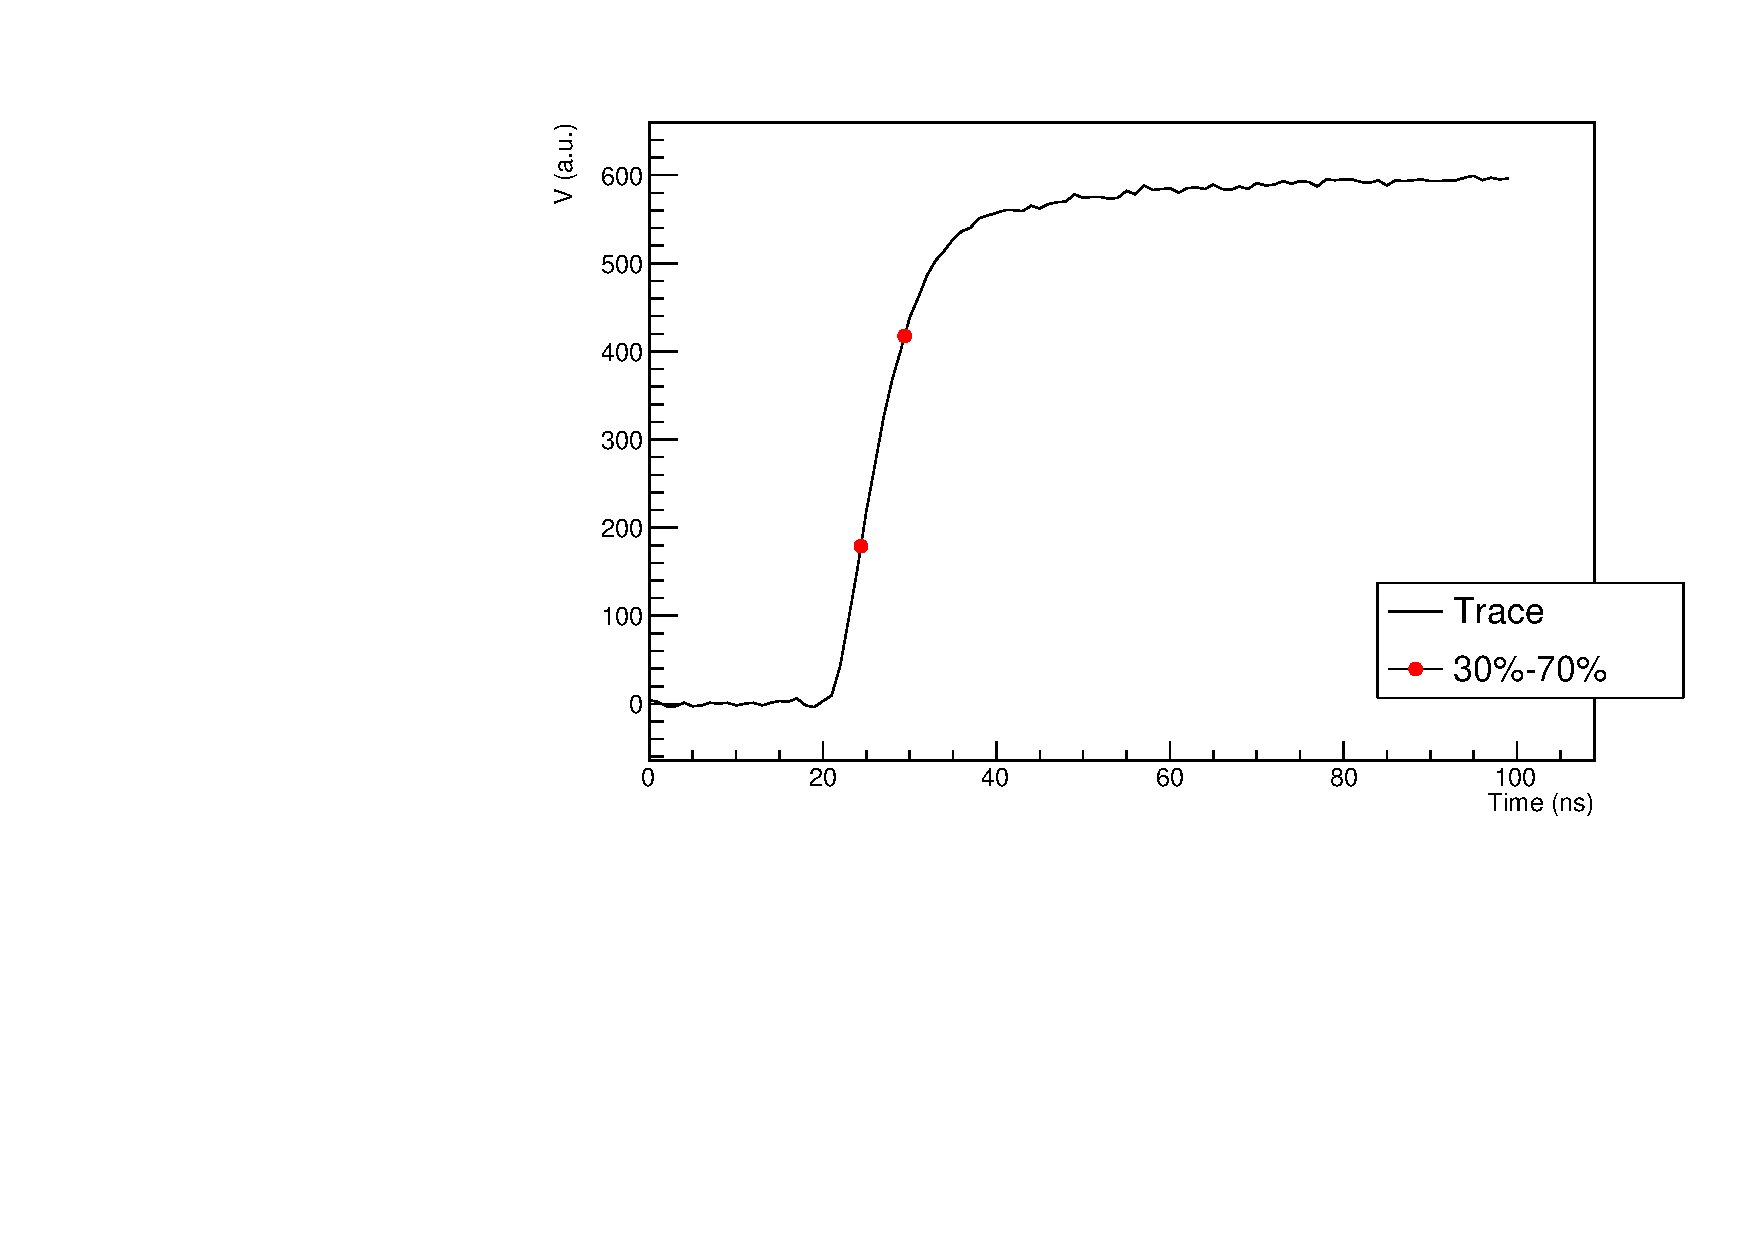
\includegraphics[scale=.6]{img/example_pulse.pdf}
  \caption{An example of the Trace pulse signal. The two points represent the $t_{0.3}$ and $t_{0.7}$.}
  \label{pulse}
\end{figure}

At the end, for each experimental run and each digitizer (the \textit{gal09}
one, and the \textit{gal10}), a TTree object, called \textit{TraceEvent}, was created with the following variables:

\begin{itemize}
\item fDomain
\item fTimeStamp
\item fSubData (vector)
  \begin{itemize}
  \item fSubDomain
  \item fEnergy
  \item fTrace
  \item fTime
  \item fBaseline
  \item fPSA
  \end{itemize}
\end{itemize}
where \textit{fDomain} is the ID of the DAQ used, \textit{fTimeStamp} is the
time given by the digitizer, \textit{fSubDomain} is the detector channel,
\textit{fEnergy} is the energy of the particle and the others are variables
filled according to the PSA: \textit{fTime} is the calculated rise time and
\textit{fTrace} is the maximum derivative of the signal (\textit{fBaseline} and
\textit{fPSA} were later used as Neural Network outputs that gives the
probability of the particle being either a proton or an alpha).

Plots of the $\tau _{\textup{rise}}$ and $i_{\textup{max}}$ in function of the energy
are shown in Fig.~\ref{imax} and Fig.~\ref{risetime}. The $\alpha$ and proton
traces are clearly visible and so they can be tagged and used for the
Neural Network construction. Moreover, even though the signals seem almost
backgroundless, many pulses are present that can not be tagged as neither a
proton nor $\alpha$. In fact, the protons stop at $\approx 4$ MeV and
$\alpha$'s at $\approx 6$ MeV as expected from detector response simulations
performed through LISE software~\cite{lise} (origins of the remaining signals
are not known).

\begin{figure}[h]
  \centering
  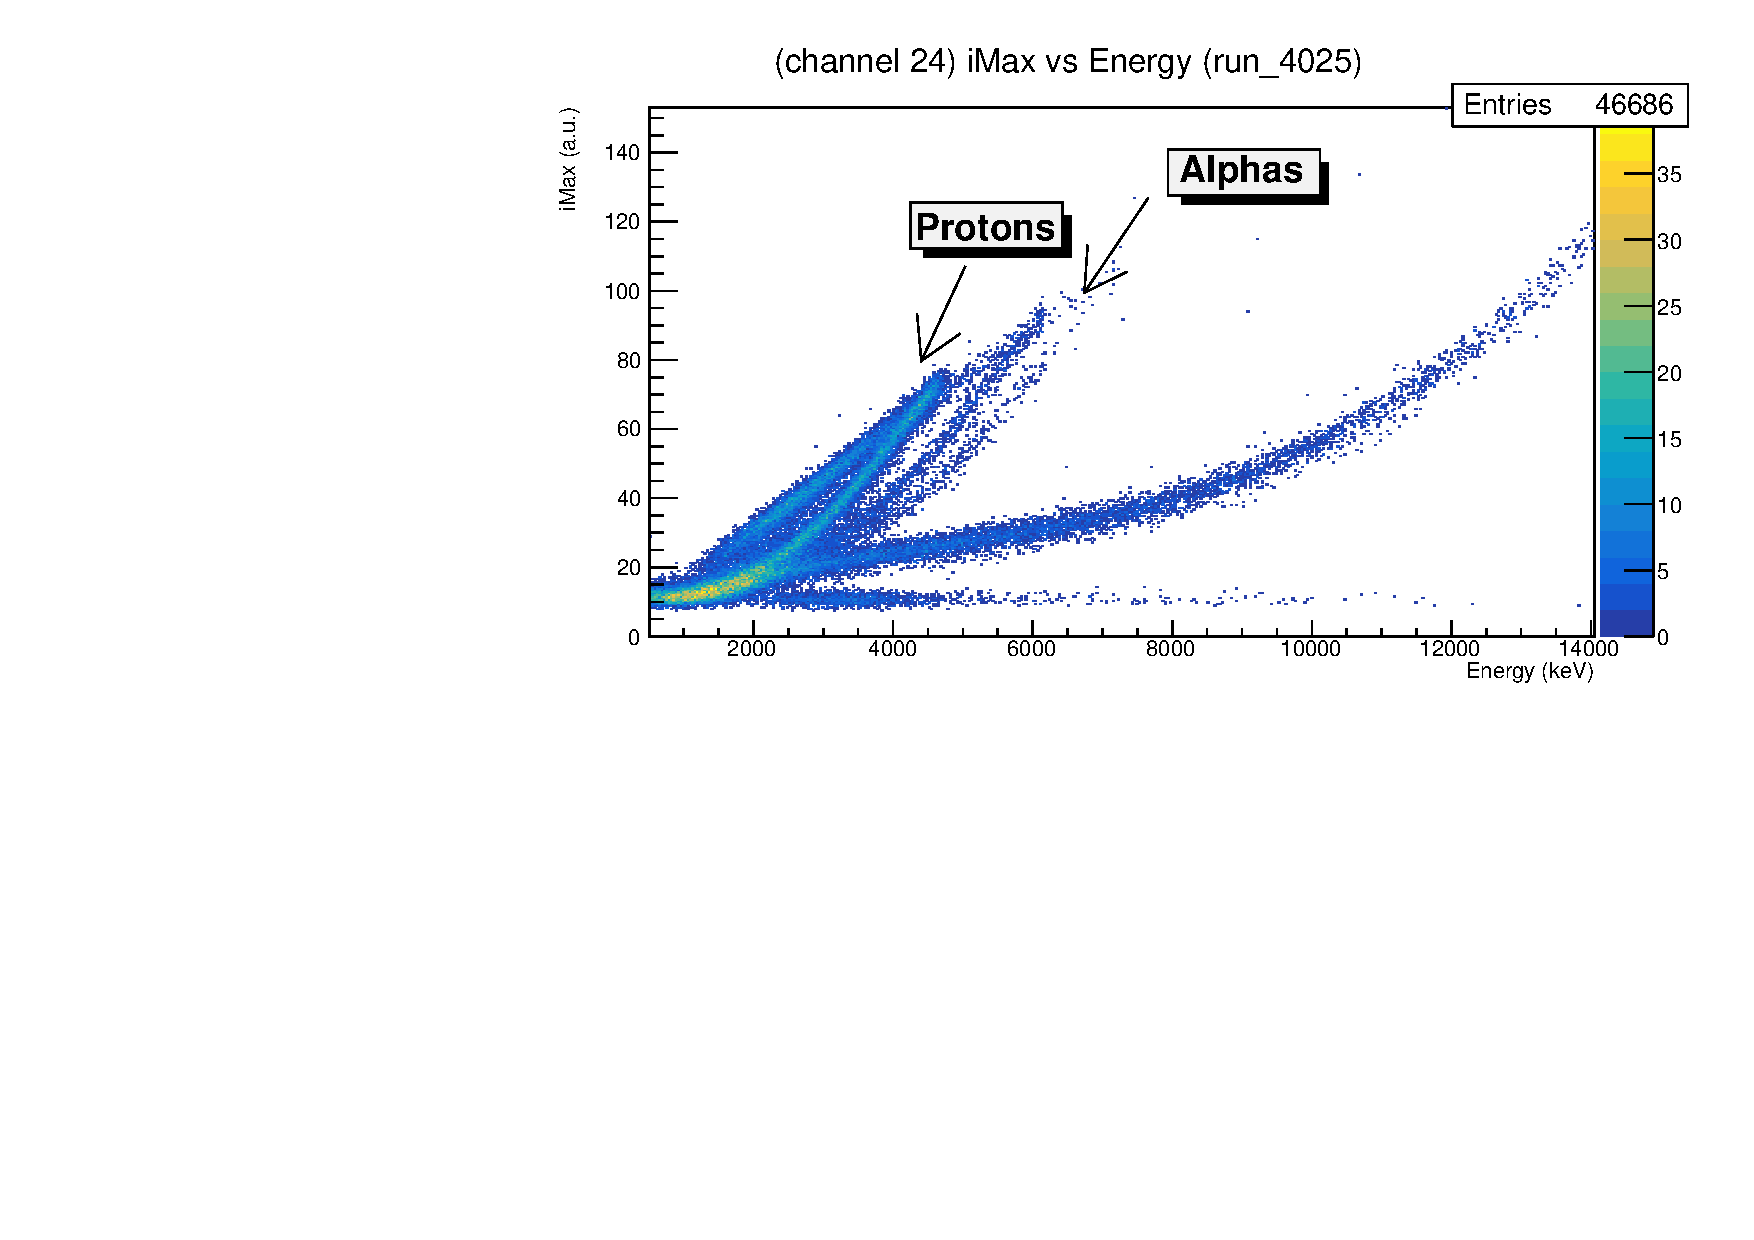
\includegraphics[scale=.6]{img/iMax_4025.pdf}
  \caption{An example of the $i_{\textup{max}}$ vs \textit{E} graph for the 4025 run (only one channel is considered).}
  \label{imax}
\end{figure}

\begin{figure}[h]
  \centering
  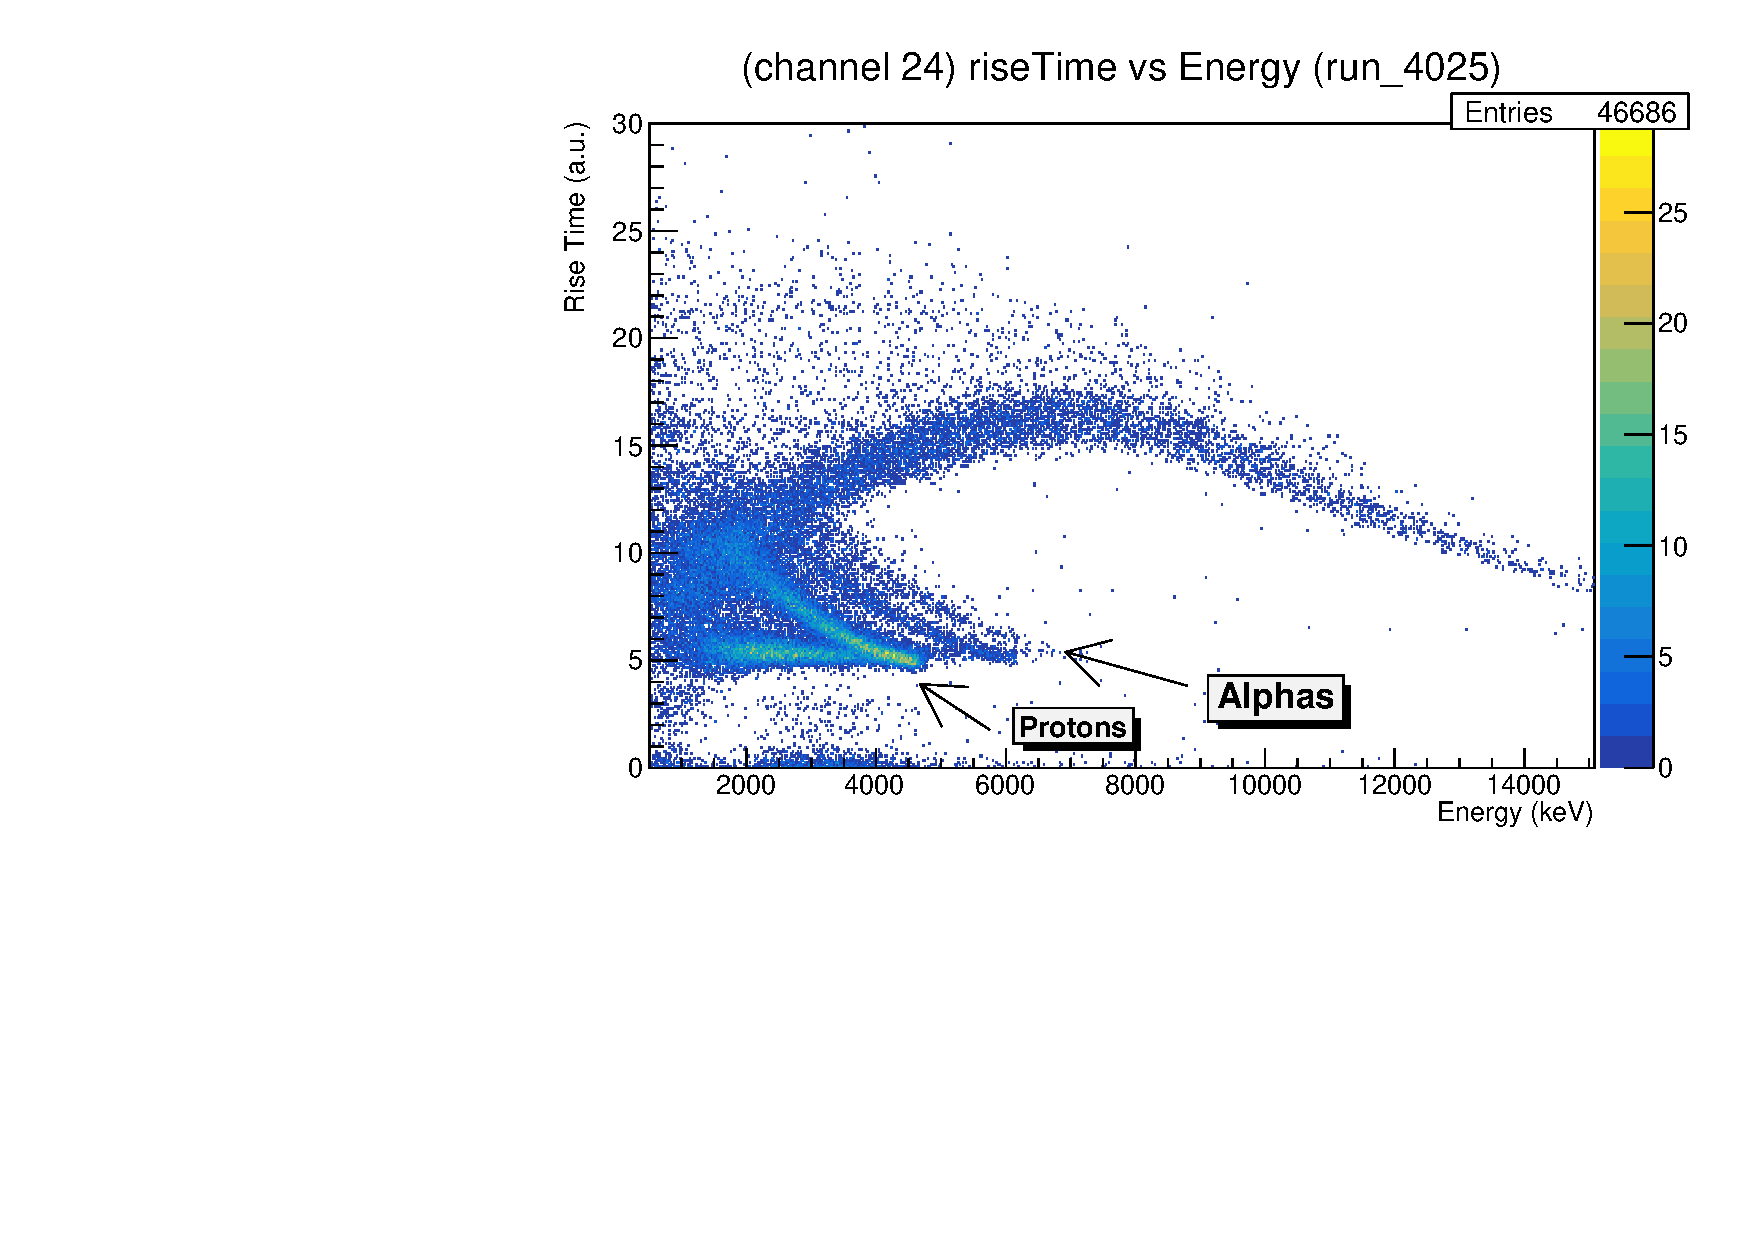
\includegraphics[scale=.6]{img/riseTime_4025.pdf}
  \caption{An example of the $\tau _{\textup{rise}}$ vs \textit{E} graph for the 4025 run (only one channel is considered).}
  \label{risetime}
\end{figure}

\subsection{Deep Learning for Pulse Shape Analysis with TRACE} \label{deep}
With the rise of user-friendly machine learning frameworks such as TensorFlow~\cite{tensorflow} or Pytorch~\cite{pytorch}, Deep Learning had seen a wide range of applications in physics~\cite{ml4phys}. In experimental nuclear and subnuclear physics pre-trained Neural Network (NN) can be used for task such as event tagging~\cite{baldi} or inside the trigger system/acquisition chain in HEP experiments~\cite{williams}. 


In this section an application of NNs to perform particle discrimination using the signals collected from the TRACE detector is presented. Such a technique can be used to improve data processing speed or implemented in the acquisition system for the future.
The code of the following analysis is available at~\cite{github-nn}.

\subsubsection{Dataset and training}

In order to train a network to discriminate between two different kinds of signals from the detector we need a dataset of labeled signals from the classes we want to distinguish. Data from the run \emph{4025} are assigned to three different classes based on cuts made in the region of the graph in Fig.~\ref{imax}, either labeled as \emph{proton}, \emph{alpha} or \emph{other}. The dataset is then balanced resulting in \num{39000} labeled input signals to train the network, \num{13000} for each class. Examples of signals are shown in Fig.~\ref{input}.

\begin{figure}[htb]
  \centering
  \begin{minipage}[b]{0.45\textwidth}
    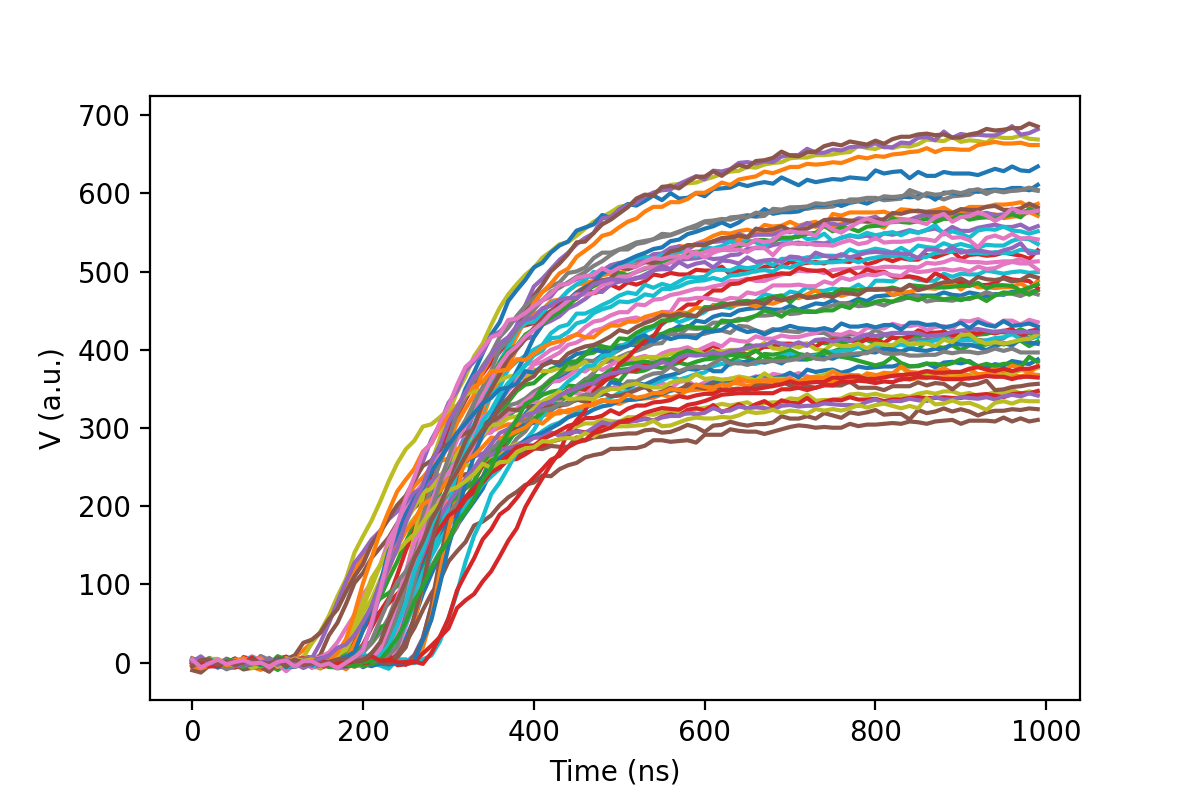
\includegraphics[width=\textwidth]{img/protons.png}
    \caption{Protons}
    %\label{}
  \end{minipage}
  \hfill
  \begin{minipage}[b]{0.45\textwidth}
   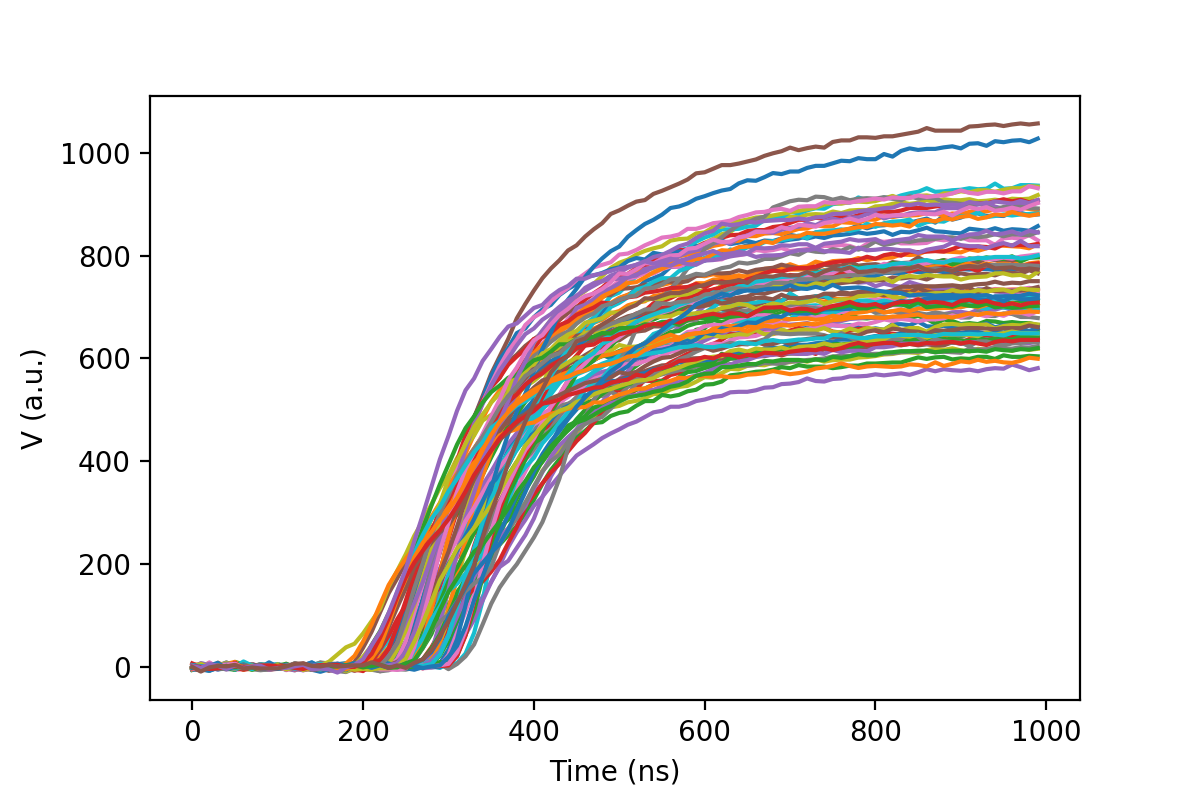
\includegraphics[width=\textwidth]{img/alpha.png}
  \caption{Alpha}
  %\label{}
  \end{minipage}
  \hfill
  \begin{minipage}[b]{0.45\textwidth}
   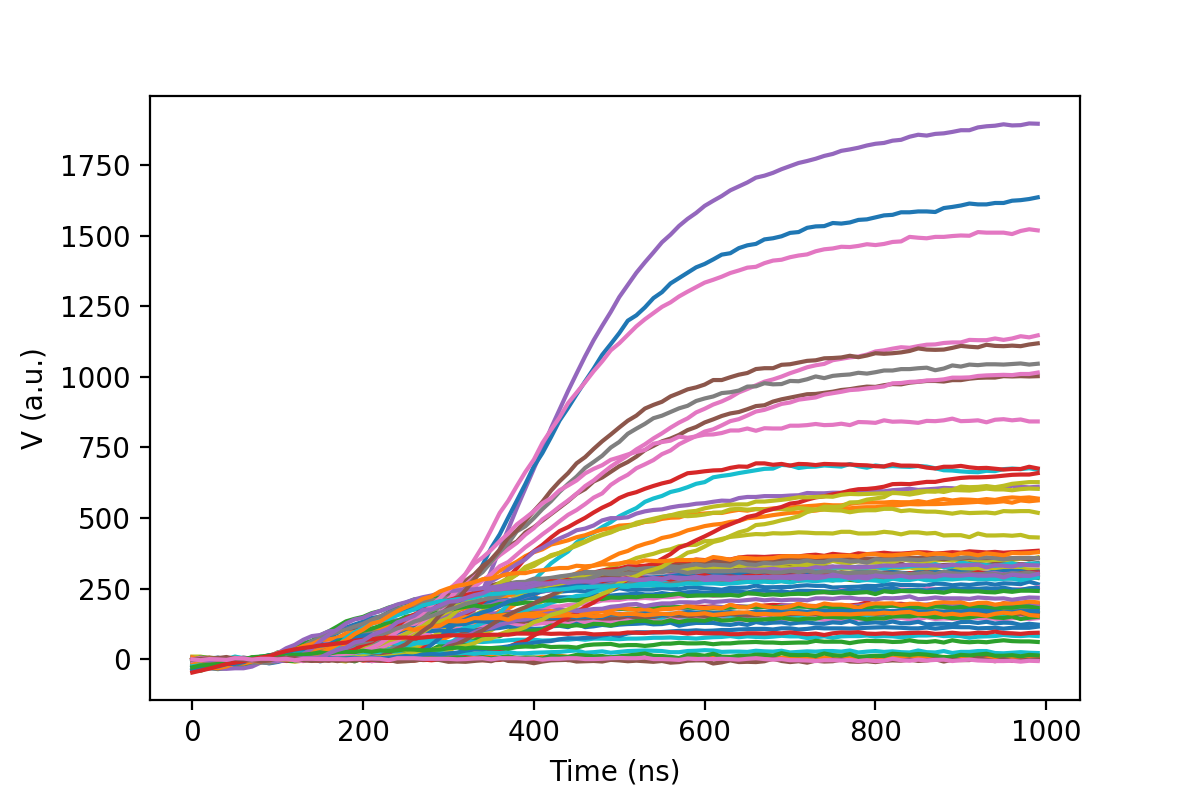
\includegraphics[width=\textwidth]{img/other.png}
  \caption{Other}
  %\label{}
  \end{minipage}
  \caption{Examples of input from the three classes.}
  \label{input}
\end{figure}

The dataset is split into the actual training data (\num{90}\%) and a set for validation (\num{10}\%). The training data are then fed to a simple feedforward NN istantiated into the framework Pytorch with the following architecture:

\begin{itemize}
	\item Input layer (The \num{100} points of the sampled signal)
	\item 2 Hidden layers of 64 units (\emph{ReLU} activation)
	\item Output layer (\emph{softmax} activation, 3 classes).
\end{itemize}

The training is performed optimizing a Mean Squared Error (MSE) function for the labels using the \emph{Adamax} optimizer. Data are given in batches of 200 samples, over several ($\sim 30$) epochs of training. At the end is possible use the model on data from other runs to try to classify it.

\subsubsection{Validation and Application of the model}

The perfomance of the network is evaluated using both the validation dataset of \num{3900} samples not used for the training and a dataset of 2960 events taken from one calibration run using an alpha source.


The maximal accuracy (percentage of events classified correctly) achievable on the testing dataset is of $\sim\num{94} \%$ with the confusion matrix shown in Fig.~\ref{conf_test}, which shows that overall no bias is present on the misclassified events.


Using the data from the calibration run an accuracy of $\sim\num{67} \%$ is achieved which is significantly lower from the former result. This is exected due to the fact that the data are taken in different condition, nonetheless the confusion matrix in Fig.~\ref{conf_alpha} shows that the NN almost never missclassify an alpha particle for a proton.

\begin{figure}[htb]
  \centering
  \begin{minipage}[b]{0.45\textwidth}
    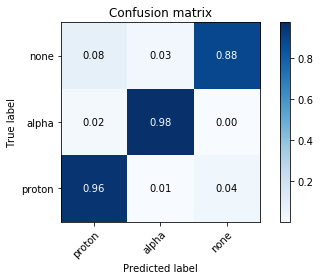
\includegraphics[width=\textwidth]{img/conf_test.png}
    \caption{Test dataset}
    \label{conf_test}
  \end{minipage}
  \hfill
  \begin{minipage}[b]{0.45\textwidth}
   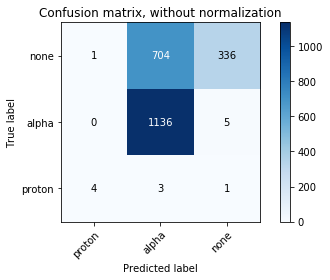
\includegraphics[width=\textwidth]{img/conf_alphas.png}
  \caption{Calibration Run}
  \label{conf_alpha}
  \end{minipage}
  \caption{Confusion matrices for the two datasets.}
  \label{input:deep}
\end{figure}

At the end of the validation the trained model is exported and implemented into a C++ program that merges the data of the previous trees with the output of the neural network. This two new entries should be interpreted as probabilities of the particle being an proton or alpha in the energy range of the particles which stop into the $\Delta E$ detector (below $\sim \num{4}/\num{6}$ MeV). 

The final ROOT TTree include the data from the GALILEO detector array. It can be used to look for coincidence between the evaporation residues from the daughter nuclei formed and $\gamma$'s emitted from the their disexcitation.







\clearpage

\section{Conclusions}

An in-depth characterization and calibration of the TRACE detector was given using an alpha source. The detector was then tested in the GALTRACE experiment at LNL. The data acquired during the different runs was then analyzed in order to reconstruct the structure of each event comprehensive of the PSA variables extracted from the raw signals from the digitizer. Fig.~\ref{imax} and Fig.~\ref{risetime} shows the plot obtained from this analysis.


The also showed that is possible to train a neural network using signals from different regions of the graph to distinguish between different types of particles (Section~\ref{deep}).


A full reconstruction of the events as well as a selection of interesting transition is behind the scope of this work, however some work was made in order to characterize the spectrum obtained by the GALILEO array coupled with the TRACE detector (Section~\ref{gammaspectr}).


\clearpage

\begin{thebibliography}{20}

\bibitem{mengoni}
  D. Mengoni et al.,
  \emph{Digital pulse-shape analysis with a TRACE early silicon prototype}, Nucl. Instrum. Meth. A764 (2014), 241-246.

\bibitem{galileo}
  D. Testov, J.J. Valiente-Dobón, D. Mengoni, F. Recchia, A. Goasduff, A. Boso, S. Lenzi, G. de Angelis, S. Lenzi et al.
  \emph{High resolution $\gamma$-ray spectroscopy using GALILEO array}, arXiv:1903.01296.
  
\bibitem{oko:cluster}
  J. Okolowicz, M. Ploszajczak and W. Nazarewicz,
  \emph{On the origin of nuclear clustering}, Prog. Theor. Phys. Supplement 196 (2012) 230.

\bibitem{oko:origin}
  J. Okolowicz, M. Ploszajczak and W. Nazarewicz,
  \emph{Toward understanding the microscopic origin of nuclear clustering}, Fortschr. Phys. 61, 66 (2013).

\bibitem{mengoni2}
  D. Mengoni,
  \emph{TRACE: a highly-segmented Silicon detector for light charged particles emitted in fusion-evaporation and direct reactions}.
  
\bibitem{strano}
  E. Strano et al., Nucl. Instrum. Methods, B317 (2013) 657.
  

\bibitem{salathe}
Salathe, Marco, and Thomas Kihm. 
\emph{Optimized Digital Filtering Techniques for Radiation Detection with HPGe Detectors}, Nucl. Instrum. Meth. A808 (2016): 150–155.

\bibitem{kuba:compa}
S. Capra, G. Benzoni, A. Compagnucci, J. M. Deltoro, J. Duenas, A. Goasduff, D. Mengoni, A. Pullia, J. Skowronski, I. Zanon, S. Ziliani, 
\emph{Validation and Charcterization of the GALTRACE Silicon Detector Array Demonstrator}.

\bibitem{tensorflow}
Martín Abadi, Ashish Agarwal, et al.
\emph{TensorFlow: Large-scale machine learning on heterogeneous systems},
2015. Software available from tensorflow.org.

\bibitem{pytorch}
Adam Paszke, Sam Gross et al.
\emph{Automatic differentiation in PyTorch},
2017

\bibitem{ml4phys}
Mehta, Pankaj et al. 
\emph{A High-Bias, Low-Variance Introduction to Machine Learning for Physicists.}, Physics Reports 810 (2019): 1–124. Crossref. Web.

\bibitem{baldi}
Baldi, Pierre, Peter Sadowski, and Daniel Whiteson, \emph{Searching for exotic particles in high-energy physics with deep learning}, Nature communications 5 (2014), 4308.

\bibitem{williams}
  Williams, J. Michael. \emph{Machine Learning in HEP}, No. LHCb-TALK-2015-338. 2015.

\bibitem{root}
  Rene Brun and Fons Rademakers,
  \emph{ROOT - An Object Oriented Data Analysis Framework}, Proceedings AIHENP'96 Workshop, Lausanne, Sep. 1996, Nucl. Inst. \& Meth. in Phys. Res. A 389 (1997) 81-86.

\bibitem{lise}
  O.B. Tarasov and D. Bazin,
  \emph{LISE++ : Exotic beam production with fragment separators and their design}, NIM B 376 (2016) 185.

\bibitem{github-nn}
  J. Skowronski \& A. Compagnucci,
  \emph{Neural Network code for GALTRACE particle discrimination} (2019), Github repository, \url{https://github.com/Alecompa/galtrace-nn}

\bibitem{charge:amp}
  A. Pullia and S. Capra,
  \emph{Experimental performance of a highly-innovative low-noise charge-sensitive preamplifier with integrated range-booster}, Journal of Instrumentation 13 (12), art. no. C12004, 2018.

\bibitem{bicmos}
  \emph{The Ams Website}, \url{https://ams.com/}

\end{thebibliography}


\end{document}
